\begin{figure*}[!h]
  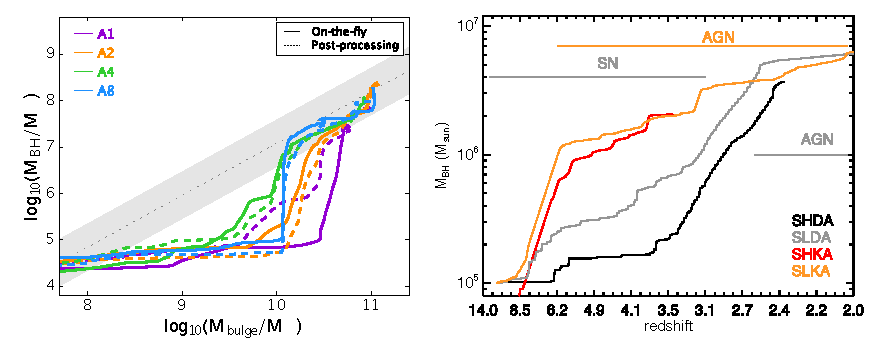
\includegraphics[width=\textwidth]{figures/comparisonfig.pdf}
    \caption{Black hole growth figures reproduced from A17 (left) and D15
    (right). For the right panel, note that the `*DA' runs use a delayed
    cooling supernovae prescription, and the `*KA' use a kinetic supernovae
    prescription. The `*SH' runs correspond to the runs performed with
    high-resolution hydrodynamics. In the left panel the different colours
    correspond to different halos, with the dashed lines showing a
    reconstructed accretion history using postprocessing of snapshots after the
    simulation. Unfortunately the data was not available scaled with the same
    property (note that on the left black hole mass is plotted with bulge mass,
    and on the right with redshift), but assuming that the bulge grows in a
    regular way with redshift both of these plots show a very similar black
    hole growth history.}
  \label{fig:bhhistory}
\end{figure*}
As mentioned in §\ref{sec:models}, there is no treatment of black holes or AGN
in the original \fire{} project. After the main runs A17 looked at the effects
of star formation on the growth of the black hole; this still did not include
any treatment of AGN feedback. The \hagn{} project, on the other hand, was
based almost entirely around the effects of AGN on galaxies and vice-versa, and
hence it is expected that their treatment is more precise.  D15 in particular
looks at the effects of star formation on black hole growth, and hence this is
directly comparable with A17.

The two projects use remarkably different models for their black hole growth.
D15 implements black hole growth using \citet{bondi_spherically_1952} such
that
\begin{align}
  \dot{M}_{BH} = 4\pi \alpha G^2 M_{BH}^2
                 \frac{\bar{\rho}}{(c_s^2 + u^2)^{3/2}},
  \label{eqn:d15:mdot}
\end{align}
where $\alpha$ is a boost factor constant, $G$ the gravitational constant,
$\bar{\rho}$ is the local mean density of gas around the black hole, $c_s$ the
local sound speed, and $u$ the average gas velocity relative to the black hole.
A17 uses the `torque' model from \citet{hopkins_analytic_2011} such that
\begin{align}
  \dot{M}_{BH} = (1 - \eta) \epsilon f_d^{5/2} M_d R_0^{-3/2} M_{BH}^{1/6}~,
  \label{eqn:a17:mdot}
\end{align}
where $f_d$ and $M_d$ are the mass fraction and total mass of the disks within
a radius of $R_0$ which encloses 256 gas particles.
Note that, due to the bulge mass-black hole mass relation
\citep{haring_black_2004}, the accretion rate essentially scales like
$\dot{M_{BH}} \propto M_{BH}^{4/3}$.

In Figure \ref{fig:bhhistory} the accretion histories of the two black holes
in both papers is shown. It is remarkable that despite very different `feeding'
models, they arrive at a very similar accretion history; this is due to the
fact that in both models, the accretion is limited by the effects of star
formation.

Both A17 and D15 show resolution depedence in their results, with the most
strong being present in D15. It also appears that for D15, the accretion
history is heavily dependent on the supernovae model used; this is attributed
to unphysical star formation in the delayed cooling model. Whilst resolution
dependence is not ideal, it is still relatively weak here and the same results
can be gleaned; at a characteristic bulge mass of around $10^{9-10}$ M$_\odot$
when the bulge and black-hole have enough mass to begin to self-regulate, the
black hole can begin to accrete at a much higher rate. At lower masses star
formation regulates the bulge mass and hence the accretion of the black hole is
quenched as excess gas is converted to stars.
